\documentclass[aspectratio=169,11pt]{beamer}

\usepackage{listings}        % code blocks
\usepackage{caption} % for \captionof



% ------- Theme (pick one) -------
\usetheme{Madrid}            % simple, built-in
% \usetheme[numbering=fraction]{metropolis} % requires the metropolis package installed

% ------- Basics -------
\usepackage[utf8]{inputenc}  % not needed if using xelatex/lualatex
\usepackage[T1]{fontenc}
\usepackage{lmodern}
\usepackage{graphicx}
\usepackage{booktabs}
\usepackage{amsmath, amsfonts}
\usepackage{listings}        % code blocks

% ------- Title info -------
\title[Short Title]{Your Talk Title}
\subtitle{Optional Subtitle}
\author{Your Name}
\institute{Your Organization}
\date{\today}

% ------- Optional tweaks -------
\setbeamertemplate{caption}[numbered]
\setbeamertemplate{footline}[frame number]
\setbeamercovered{transparent}

% ------- Document -------
\begin{document}

\begin{frame}
  \titlepage
\end{frame}

\begin{frame}{Agenda}
  \tableofcontents
\end{frame}

\section{Introduction}
\begin{frame}{Why This Matters}
  \begin{itemize}
    \item First key point
    \item Second key point \pause
    \item \alert{Callout or emphasis}
  \end{itemize}
\end{frame}

\section{Methods}
\begin{frame}{A Little Math}
  We minimize:
  \[
    J(\theta)=\sum_{i=1}^{n}\big(y_i - \theta^\top x_i\big)^2
  \]
\end{frame}

\begin{frame}{Two Columns}
  \begin{columns}[T,totalwidth=\textwidth]
    \column{0.55\textwidth}
      \begin{block}{Left Block}
        Bullets, equations, etc.
      \end{block}
    \column{0.45\textwidth}
      \begin{exampleblock}{Right Block}
        \begin{itemize}
          \item Example item
        \end{itemize}
      \end{exampleblock}
  \end{columns}
\end{frame}

\section{Results}
\begin{frame}{Figure + Table}
    \begin{figure}
        \centering
        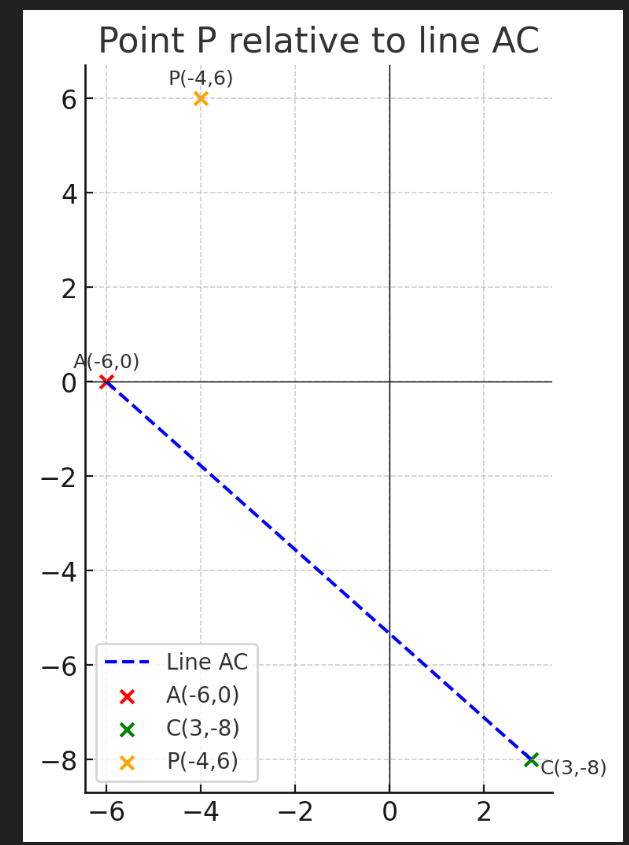
\includegraphics[width=0.3\linewidth]{Fig1.png}
        \caption{Caption}
        \label{fig:placeholder}
    \end{figure}
  \begin{minipage}{0.4\textwidth}
    \begin{tabular}{lrr}
      \toprule
      Item & A & B \\
      \midrule
      Foo  & 1 & 2 \\
      Bar  & 3 & 4 \\
      \bottomrule
    \end{tabular}
  \end{minipage}
\end{frame}


\section{Code}
\begin{frame}[fragile]{Code Listing}
\begin{lstlisting}[language=Python,basicstyle=\ttfamily\small,frame=single]
def greet(name):
    return f"Hello, {name}!"
print(greet("Beamer"))
\end{lstlisting}
\end{frame}

\section{Conclusion}
\begin{frame}{Takeaways}
  \begin{enumerate}
    \item Key takeaway 1
    \item Key takeaway 2
  \end{enumerate}
\end{frame}

\begin{frame}{Q \& A}
  \centering
  \Huge Questions?
\end{frame}

\end{document}









